\documentclass{standalone}
\usepackage{tikz}
\usetikzlibrary{patterns, positioning}
\usetikzlibrary{shapes.misc}
\usepackage[outline]{contour}
\contourlength{1.5pt} 
\usepackage[sfdefault]{ClearSans} %% option 'sfdefault' activates Clear Sans as the default text font
\usepackage[T1]{fontenc}

\begin{document}
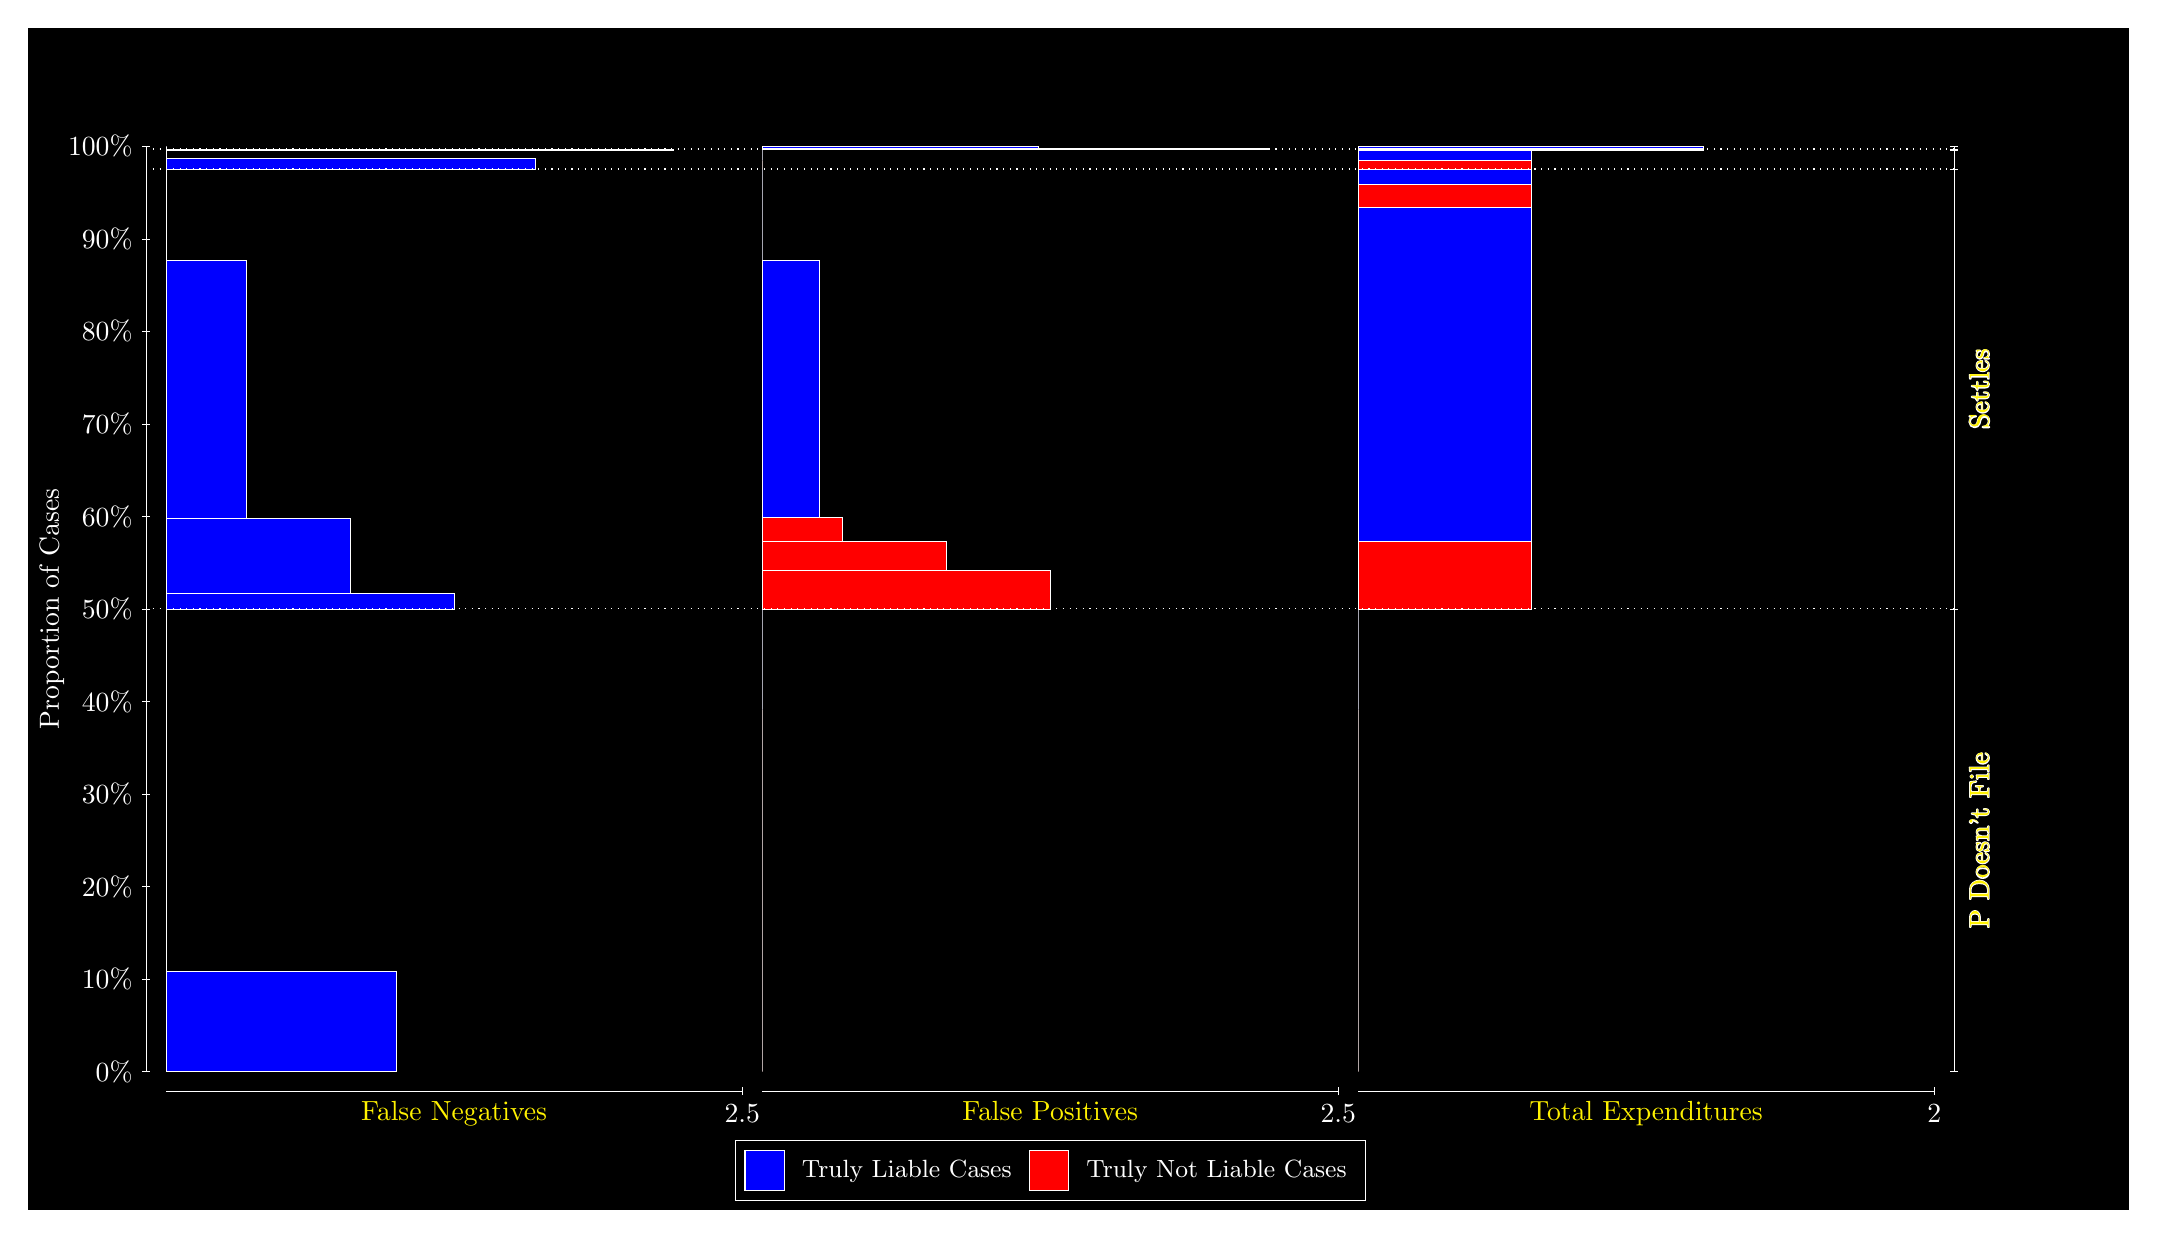
\begin{tikzpicture}
\draw[fill=black] (0,0) rectangle (26.667,15);
\draw[white, very thin] (1.5,1.75) -- (1.5,13.5);
\node[rotate=90, text=white, anchor=center] at (0.3, 7.625) {Proportion of Cases};
\draw[white, very thin] (1.45,1.75) -- (1.55,1.75);
\node[text=white, anchor=east] at (1.45, 1.75) {0\%};
\draw[white, very thin] (1.45,2.925) -- (1.55,2.925);
\node[text=white, anchor=east] at (1.45, 2.925) {10\%};
\draw[white, very thin] (1.45,4.1) -- (1.55,4.1);
\node[text=white, anchor=east] at (1.45, 4.1) {20\%};
\draw[white, very thin] (1.45,5.275) -- (1.55,5.275);
\node[text=white, anchor=east] at (1.45, 5.275) {30\%};
\draw[white, very thin] (1.45,6.45) -- (1.55,6.45);
\node[text=white, anchor=east] at (1.45, 6.45) {40\%};
\draw[white, very thin] (1.45,7.625) -- (1.55,7.625);
\node[text=white, anchor=east] at (1.45, 7.625) {50\%};
\draw[white, very thin] (1.45,8.8) -- (1.55,8.8);
\node[text=white, anchor=east] at (1.45, 8.8) {60\%};
\draw[white, very thin] (1.45,9.975) -- (1.55,9.975);
\node[text=white, anchor=east] at (1.45, 9.975) {70\%};
\draw[white, very thin] (1.45,11.15) -- (1.55,11.15);
\node[text=white, anchor=east] at (1.45, 11.15) {80\%};
\draw[white, very thin] (1.45,12.325) -- (1.55,12.325);
\node[text=white, anchor=east] at (1.45, 12.325) {90\%};
\draw[white, very thin] (1.45,13.5) -- (1.55,13.5);
\node[text=white, anchor=east] at (1.45, 13.5) {100\%};

\draw[white, very thin] (24.457,1.75) -- (24.457,13.5);
\draw[white, very thin] (24.407,1.75) -- (24.507,1.75);
\node[anchor=west] at (24.407, 1.75) {};
\draw[white, very thin] (24.407,7.625) -- (24.507,7.625);
\node[anchor=west] at (24.407, 7.625) {};
\draw[white, very thin] (24.407,13.212) -- (24.507,13.212);
\node[anchor=west] at (24.407, 13.212) {};
\draw[white, very thin] (24.407,13.456) -- (24.507,13.456);
\node[anchor=west] at (24.407, 13.456) {};
\draw[white, very thin] (24.407,13.466) -- (24.507,13.466);
\node[anchor=west] at (24.407, 13.466) {};
\draw[white, very thin] (24.407,13.5) -- (24.507,13.5);
\node[anchor=west] at (24.407, 13.5) {};

\draw[white, very thin, fill=blue] (1.75,1.75) rectangle (4.6775,3.0287);
\draw[white, very thin, fill=red] (1.75,3.0287) rectangle (1.75,7.625);
\draw[white, very thin, fill=blue] (1.75,7.625) rectangle (5.4094,7.8201);
\draw[white, very thin, fill=blue] (1.75,7.8201) rectangle (4.092,8.7822);
\draw[white, very thin, fill=blue] (1.75,8.7822) rectangle (2.7746,12.053);
\draw[white, very thin, fill=red] (1.75,12.053) rectangle (1.75,13.212);
\draw[white, very thin, fill=blue] (1.75,13.212) rectangle (6.4341,13.349);
\draw[white, very thin, fill=red] (1.75,13.349) rectangle (1.75,13.456);
\draw[white, very thin, fill=blue] (1.75,13.456) rectangle (8.1906,13.461);
\draw[white, very thin, fill=red] (1.75,13.461) rectangle (1.75,13.466);
\draw[white, very thin, fill=red] (1.75,13.466) rectangle (1.75,13.474);
\draw[white, very thin, fill=blue] (1.75,13.474) rectangle (1.75,13.5);
\draw[white, very thin, fill=red] (9.3189,1.75) rectangle (9.3189,6.3463);
\draw[white, very thin, fill=blue] (9.3189,6.3463) rectangle (9.3189,7.625);
\draw[white, very thin, fill=red] (9.3189,7.625) rectangle (12.978,8.1177);
\draw[white, very thin, fill=red] (9.3189,8.1177) rectangle (11.661,8.4899);
\draw[white, very thin, fill=red] (9.3189,8.4899) rectangle (10.344,8.784);
\draw[white, very thin, fill=blue] (9.3189,8.784) rectangle (10.051,12.055);
\draw[white, very thin, fill=blue] (9.3189,12.055) rectangle (9.3189,13.212);
\draw[white, very thin, fill=red] (9.3189,13.212) rectangle (9.3189,13.32);
\draw[white, very thin, fill=blue] (9.3189,13.32) rectangle (9.3189,13.456);
\draw[white, very thin, fill=red] (9.3189,13.456) rectangle (9.3189,13.46);
\draw[white, very thin, fill=blue] (9.3189,13.46) rectangle (9.3189,13.466);
\draw[white, very thin, fill=red] (9.3189,13.466) rectangle (15.759,13.474);
\draw[white, very thin, fill=blue] (9.3189,13.474) rectangle (12.832,13.5);
\draw[white, very thin, fill=red] (16.888,1.75) rectangle (16.888,6.3463);
\draw[white, very thin, fill=blue] (16.888,6.3463) rectangle (16.888,7.625);
\draw[white, very thin, fill=red] (16.888,7.625) rectangle (19.083,8.4899);
\draw[white, very thin, fill=blue] (16.888,8.4899) rectangle (19.083,12.723);
\draw[white, very thin, fill=red] (16.888,12.723) rectangle (19.083,13.017);
\draw[white, very thin, fill=blue] (16.888,13.017) rectangle (19.083,13.212);
\draw[white, very thin, fill=red] (16.888,13.212) rectangle (19.083,13.32);
\draw[white, very thin, fill=blue] (16.888,13.32) rectangle (19.083,13.456);
\draw[white, very thin, fill=red] (16.888,13.456) rectangle (21.279,13.46);
\draw[white, very thin, fill=blue] (16.888,13.46) rectangle (21.279,13.466);
\draw[white, very thin, fill=red] (16.888,13.466) rectangle (21.279,13.474);
\draw[white, very thin, fill=blue] (16.888,13.474) rectangle (21.279,13.5);
\draw[white, dotted] (1.5,7.625) -- (24.457,7.625);
\draw[white, dotted] (1.5,13.212) -- (24.457,13.212);
\draw[white, dotted] (1.5,13.456) -- (24.457,13.456);
\draw[white, dotted] (1.5,13.466) -- (24.457,13.466);
\draw[white, very thin] (1.75,1.5) -- (9.0689,1.5);
\node[text=yellow, anchor=north] at (5.4094, 1.5) {False Negatives};
\draw[white, very thin] (9.0689,1.45) -- (9.0689,1.55);
\node[text=white, anchor=north] at (9.0689, 1.45) {2.5};

\draw[white, very thin] (9.3189,1.5) -- (16.638,1.5);
\node[text=yellow, anchor=north] at (12.978, 1.5) {False Positives};
\draw[white, very thin] (16.638,1.45) -- (16.638,1.55);
\node[text=white, anchor=north] at (16.638, 1.45) {2.5};

\draw[white, very thin] (16.888,1.5) -- (24.207,1.5);
\node[text=yellow, anchor=north] at (20.547, 1.5) {Total Expenditures};
\draw[white, very thin] (24.207,1.45) -- (24.207,1.55);
\node[text=white, anchor=north] at (24.207, 1.45) {2};

\node[text=yellow, centered, rotate=90] at (24.777, 4.6875) {\contour{white}{P Doesn't File}};
\node[text=yellow, centered, rotate=90] at (24.777, 10.419) {\contour{white}{Settles}};




\draw (12.978300999999998,1.5) node[draw=none] (baseCoordinate) {};
\begin{scope}[align=center]
        \matrix[scale=0.5, draw=white, below=0.5cm of baseCoordinate, nodes={draw}, column sep=0.1cm]{
            \node[rectangle, draw, minimum width=0.5cm, minimum height=0.5cm, fill=blue] {}; &
            \node[draw=none, font=\small, text=white] (B) {Truly Liable Cases}; &
            \node[rectangle, draw, minimum width=0.5cm, minimum height=0.5cm, fill=red] {}; &
            \node[draw=none, font=\small, text=white] (B) {Truly Not Liable Cases}; \\
            };
\end{scope}

\end{tikzpicture}
\end{document}